\documentclass[conference]{IEEEtran}
\IEEEoverridecommandlockouts
% The preceding line is only needed to identify funding in the first footnote. If that is unneeded, please comment it out.
\usepackage{cite}
\usepackage{amsmath,amssymb,amsfonts}
%\usepackage{algorithmic}
\usepackage{algorithm}
\usepackage{algpseudocode}
\usepackage{subfigure}
\usepackage{graphicx}
\usepackage{textcomp}
\usepackage{float}
\usepackage{tabu}
\def\BibTeX{{\rm B\kern-.05em{\sc i\kern-.025em b}\kern-.08em
    T\kern-.1667em\lower.7ex\hbox{E}\kern-.125emX}}
\begin{document}

\title{Paper Title*\\
{\footnotesize \textsuperscript{*}Note: Sub-titles are not captured in Xplore and
should not be used}
\thanks{Identify applicable funding agency here. If none, delete this.}
}

\author{\IEEEauthorblockN{1\textsuperscript{st} Given Name Surname}
\IEEEauthorblockA{\textit{dept. name of organization (of Aff.)} \\
\textit{name of organization (of Aff.)}\\
City, Country \\
email address}
\and
\IEEEauthorblockN{2\textsuperscript{nd} Given Name Surname}
\IEEEauthorblockA{\textit{dept. name of organization (of Aff.)} \\
\textit{name of organization (of Aff.)}\\
City, Country \\
email address}
\and
\IEEEauthorblockN{3\textsuperscript{rd} Given Name Surname}
\IEEEauthorblockA{\textit{dept. name of organization (of Aff.)} \\
\textit{name of organization (of Aff.)}\\
City, Country \\
email address}
\and
\IEEEauthorblockN{4\textsuperscript{th} Given Name Surname}
\IEEEauthorblockA{\textit{dept. name of organization (of Aff.)} \\
\textit{name of organization (of Aff.)}\\
City, Country \\
email address}
\and
\IEEEauthorblockN{5\textsuperscript{th} Given Name Surname}
\IEEEauthorblockA{\textit{dept. name of organization (of Aff.)} \\
\textit{name of organization (of Aff.)}\\
City, Country \\
email address}
\and
\IEEEauthorblockN{6\textsuperscript{th} Given Name Surname}
\IEEEauthorblockA{\textit{dept. name of organization (of Aff.)} \\
\textit{name of organization (of Aff.)}\\
City, Country \\
email address}
}

\maketitle

\begin{abstract}

Users face location-privacy risks when accessing Location-Based Services (LBSs) in an Opportunistic Mobile Social Networks (OMSNs). In order to protect the original requester's identity and location, we propose a location privacy obfuscation protocols, called Appointment Card Protocol (ACP), utilizing social ties between users. To facilitate the obfuscation operations of queries, we introduce the concept called Appointment Card (AC). The original requesters can send their queries to the LBS directly using the information in the AC, ensuring that the original requester is not detected by the LBS. Also, a path for reply message is kept when the query is sent, to help reduce the time for replying queries. Simulation results show that our protocol has a higher query success ratio than its counterparts.

\end{abstract}

\begin{IEEEkeywords}
obfuscation, encryption, location-privacy, opportunistic mobile social networks
\end{IEEEkeywords}

\section{Introduction}

The Opportunistic Mobile Social Networks (OMSN) is defined ``as decentralized opportunistic communication networks formed among human carried mobile devices that take advantage of mobility and social networks to create new opportunities for exchanging information and mobile ad hoc social networking'' \cite {C24}. People carrying smartphones which contain WiFi or Bluetooth can form a typical OMSN, which can also be viewed as a kind of Delay Tolerant Networks (DTNs) \cite {C1} featuring lack of continuous connectivity. More specifically, in OMSNs, it is not necessary for senders to have an end-to-end routing path to their destinations. Users make contact when they encounter each other. 

Location-privacy is becoming a major concern in OMSN.  Location-Based Services (LBSs) are common applications in OMSNs, and they are widely used in ``military and government industries, emergency services and the commercial sector'' \cite {C2}, especially after the proliferation of localization technologies, like GPS. Many people access LBSs with their portable devices and send their location to LBS providers. In this case, LBS users face a constant risk that their location may be leaked from LBS applications. That makes people unwilling to use LBSs. Thus, protecting location privacy has been a critical issue in LBSs.

It is apparent that you must reveal your location if you use LBS. When you use an LBS application to find the nearest restaurant, you actually tell the LBS provider your location and your next destination which might have a restaurant nearby. If attackers can access the LBS provider's database, they can learn that information. Then you may receive many advertisements from surrounding restaurants. Such inference attack, in addition to bothering you with advertisements, can become more dangerous when you send more queries to the LBS provider. If you use the former LBS application several times in a day, attackers can learn your trace from the information so that they can infer more information including your identity and home address \cite {C23}.

Early location privacy protection methods, such as obfuscation algorithms, generate anonymized areas for the original LBS requesters so that the requesters are mixed with a group of other LBS users \cite{C3} \cite{C21}. Users send an anonymized area instead of their exact coordinate to the LBS providers when launching an LBS request. After that, social ties are incorporated into obfuscation algorithms to improve or protect location privacy. For example, the authors in \cite{C4} use social ties to determine trustable friends who could be chosen as intermediaries to forward obfuscation queries. The authors in \cite{C5} and \cite{C6} present algorithms which aim at improving delivery performance. These papers assume that attackers can access the LBS servers, which enables them to learn LBS users’ identities and locations. If a user sends a query to an LBS server with his real identity and location (e.g., a query asking for a path from his current location to a certain place), attackers can locate the user quite easily. Therefore, hiding the original requester’s real identity and the location is the focus of our work.

Inspired by \cite{5} and \cite{C7} which use the social network for messages forwarding in mobile ad hoc networks, we propose a distributed location-privacy algorithm, called ACP, which aims to guarantee location-privacy and reach a higher query success ratio. The introduction of social networks enables us to hide the original requester's information behind his friends. We introduce the Appointment Card (AC) as a kind of intermediary which records a serial of agents. The original requester sends his query using the identity of the first agent in the AC to the LBS, which prevent the LBS learns the identity of the requester. The reply of the query can be delivered back to the original requester along with the same serial of agents as in the AC one by one. The last agent called the trusted agent is a user in the social network of the original requester, in other words, he is a friend (or a friend of friends) of the original requester. The trusted agent separates the stranger-agents and the original requester so that no stranger knows the identity of the original requester. The query-delivery success ratio of the ACP is in a similar level as the no-privacy protocol comparison in our experiment.

The rest of this paper is organized as follows. Section \ref{RelatedWork} presents some related protocols in privacy-protection. The process of ACP is described in Section \ref{AppCrdPrl}. Experimental results are provided Section \ref{Experiment} followed by some concluding remarks.

\section{Related Work} \label{RelatedWork}

Users face risks of information breach when they access a semi-trusted LBS provider, because anyone who has access to data in LBSs is able to steal and misuse LBS users’ location-privacy. Considering that  LBSs rely on location-aware computing, it is unavoidable to leak users' location from LBSs. Therefore, balancing “these two competing aims of location privacy and location awareness” \cite{C8} is always a challenge.

Some early solutions, like \cite{C9} and \cite{C3}, generate a specific area based on k-anonymity \cite{C10} for each user who needs to send queries. For example, \cite{C9} gives a rectangle as an anonymized area, in which all nodes form a group to hide the original requester. But, it requires at least k connected agents to complete its obfuscation process. \cite{C3} uses a central anonymity server as a mix router. As a result, it is necessary for each node to have a continuous connection to the server. That is hard to achieve in a sparse DTN. With a similar problem as in \cite{C3}, \cite{C11} employs a matchmaker which is used to match users and advertisements, then users can achieve anonymization of their identities and locations from the matchmaker. However, the matchmaker is a high-risk in the network, because it collects so much private information. In the work in \cite{C12}, exact locations and requests from clients are replaced by a location anonymization engine before they arrive at LBS providers. Since the anonymization engine learns all exact locations and requests, it becomes a better target for malicious attack.

There are protocols with more servers. The servers are settled in the network and each one of them takes charge of a certain area. \cite{C13} uses roadside units (RSUs) as mix servers in a vehicular DTN, and the destination is encrypted during forwarding, so eavesdropping queries cannot help attackers to locate users. But deploying the RSUs is not always feasible. In \cite{C21}, sensor nodes which are scattered throughout the network provide anonymized locations for users. Since the sensor nodes’ coverage should possess a non-overlapping characteristic, it is difficult to deploy them in real-world. Besides, the mix servers and sensor nodes might be more prominent targets than LBS providers.

However, the system could also be a distributed one, like protocols SLPD \cite{C4}, Hybrid and Social-aware Location-Privacy in Opportunistic mobile social networks (HSLPO) \cite{C5} and Location Privacy-Aware Forwarding (LPAF) \cite{C6}. The obfuscation processes are performed by each separated node independently without any help from a third-party device. The SLPD is the basic version of the above three protocols, in which authors use two phases: the obfuscation phase and the free phase. A query from an original requester always starts in the obfuscation phase and passes through k friends. For example, the original requester sends the query to one of his friend in one hop, and then the friend forwards the query to another friend. We call these friends the agents. That process repeats for exactly $k$ times. When the kth friend gets the query, he switches the query to the free phase and replaces the sender identity with his own identity, and then sends the query to the destination (e.g., LBS) using any DTN protocol. The disadvantage of the protocol is that it is hard to encounter a friend in the network, which can decrease the success ratio for the queries. When there are only a few friends in the network, it is hard for a node to find an available next hop in obfuscation phase. HSLPO tries to improve the delivery performance by using a stochastic model for location prediction. The dominant process is similar to that in SLPD, but an agent can forward the query to a user who is not a friend of the original requester if the user has more chance to deliver the query and a trust value is larger than a threshold. LPAF also attempts to improve SLPD’s performance in a way that some ineligible users in SLPD are chosen as friends based on the additional requirements. The protocol Social-aware Location-privacy Protection (SLP) \cite{C20} also uses  social tie to protect the privacy of the original requester and uses cloaking areas instead of the exact coordinates to enhance security, but the original requester still must take the risk that strangers might learn everything of the query.

\section{Appointment Card Protocol} \label{AppCrdPrl}

\subsection{System Model}

The network architecture consists of two main classes of entities: Users and Location-Based Service Providers (LBSPs). Users are mobile and communicate with others within a certain range, i.e., the communication range of their portable devices. For a given user, other users in the social network are either strangers or his friends whom he can detect when they are in his communication range. Let ${RS}_{i,j}$ denote the relationship strength \cite{C18} between user $i$ and $j$. If ${RS}_{i,j}$ is larger than a specific threshold, ${FT}_{min}$, user $j$ is considered a friend of $i$. LBSPs, which provide location-based services to the users are fixed and not part of the social network. We assume that the only information which is necessary for the LBSP is a location from the original requester, but the original requester should still give an identity to the LBSP so that the LBSP can reply to that identity.

We consider external attacker capable of eavesdropping on limited traffic in the network. We assume that the attacker can access the database of LBSPs, so that he can learn everything recorded in LBSP's memory, including user identities and locations. The attacker launches an inference attack on each user who uses the LBS in an attempt to learn user's private information based on location and context in the queries. Therefore, the key to protecting location-privacy is degrading the relationship between the user identity and the location provided by him so that the attacker can hardly infer the identity of the original requester by the known information. 

We propose ACP to protect the identity and location-privacy of the original requester by providing other users' identity (agents), which can be any user in the network so that ACP can have a large anonymity set. The friends of the original requester separate the agents and the original requester so that the agents have no knowledge about the original requester.


\subsection{ Appointment Card Protocol Overview} \label{AppCrdPrlOver}

Our proposed ACP protects original requesters when they are served by LBSPs. A user (${Agt}_{1}$) generates his own Appointment Cards (ACs) containing his own identity called $Cid$ and a unique number called $Capt$ (a number generated by the creator of AC). The ACs are exchanged when two users encounter each other. When the original requester sends a query, he chooses an AC and sends the query using the identity ${Agt}_{1}$ of the first agent which is in the AC. The LBSP replies to ${Agt}_{1}$ when it receives the query. ${Agt}_{1}$ is the one who has generated the AC and the first agent of the AC. ${Agt}_{1}$ then forwards the reply to the next agent (${Agt}_{2}$) who already has received AC from him, and so on until the reply reaches the last agent. The last agent is responsible for forwarding it to the original requester. Therefore, we can consider the ACP as two parts: 1. users generate and exchange ACs continously; 2. users use ACs when they want to send a query.

\begin{figure*}
  \centering 
  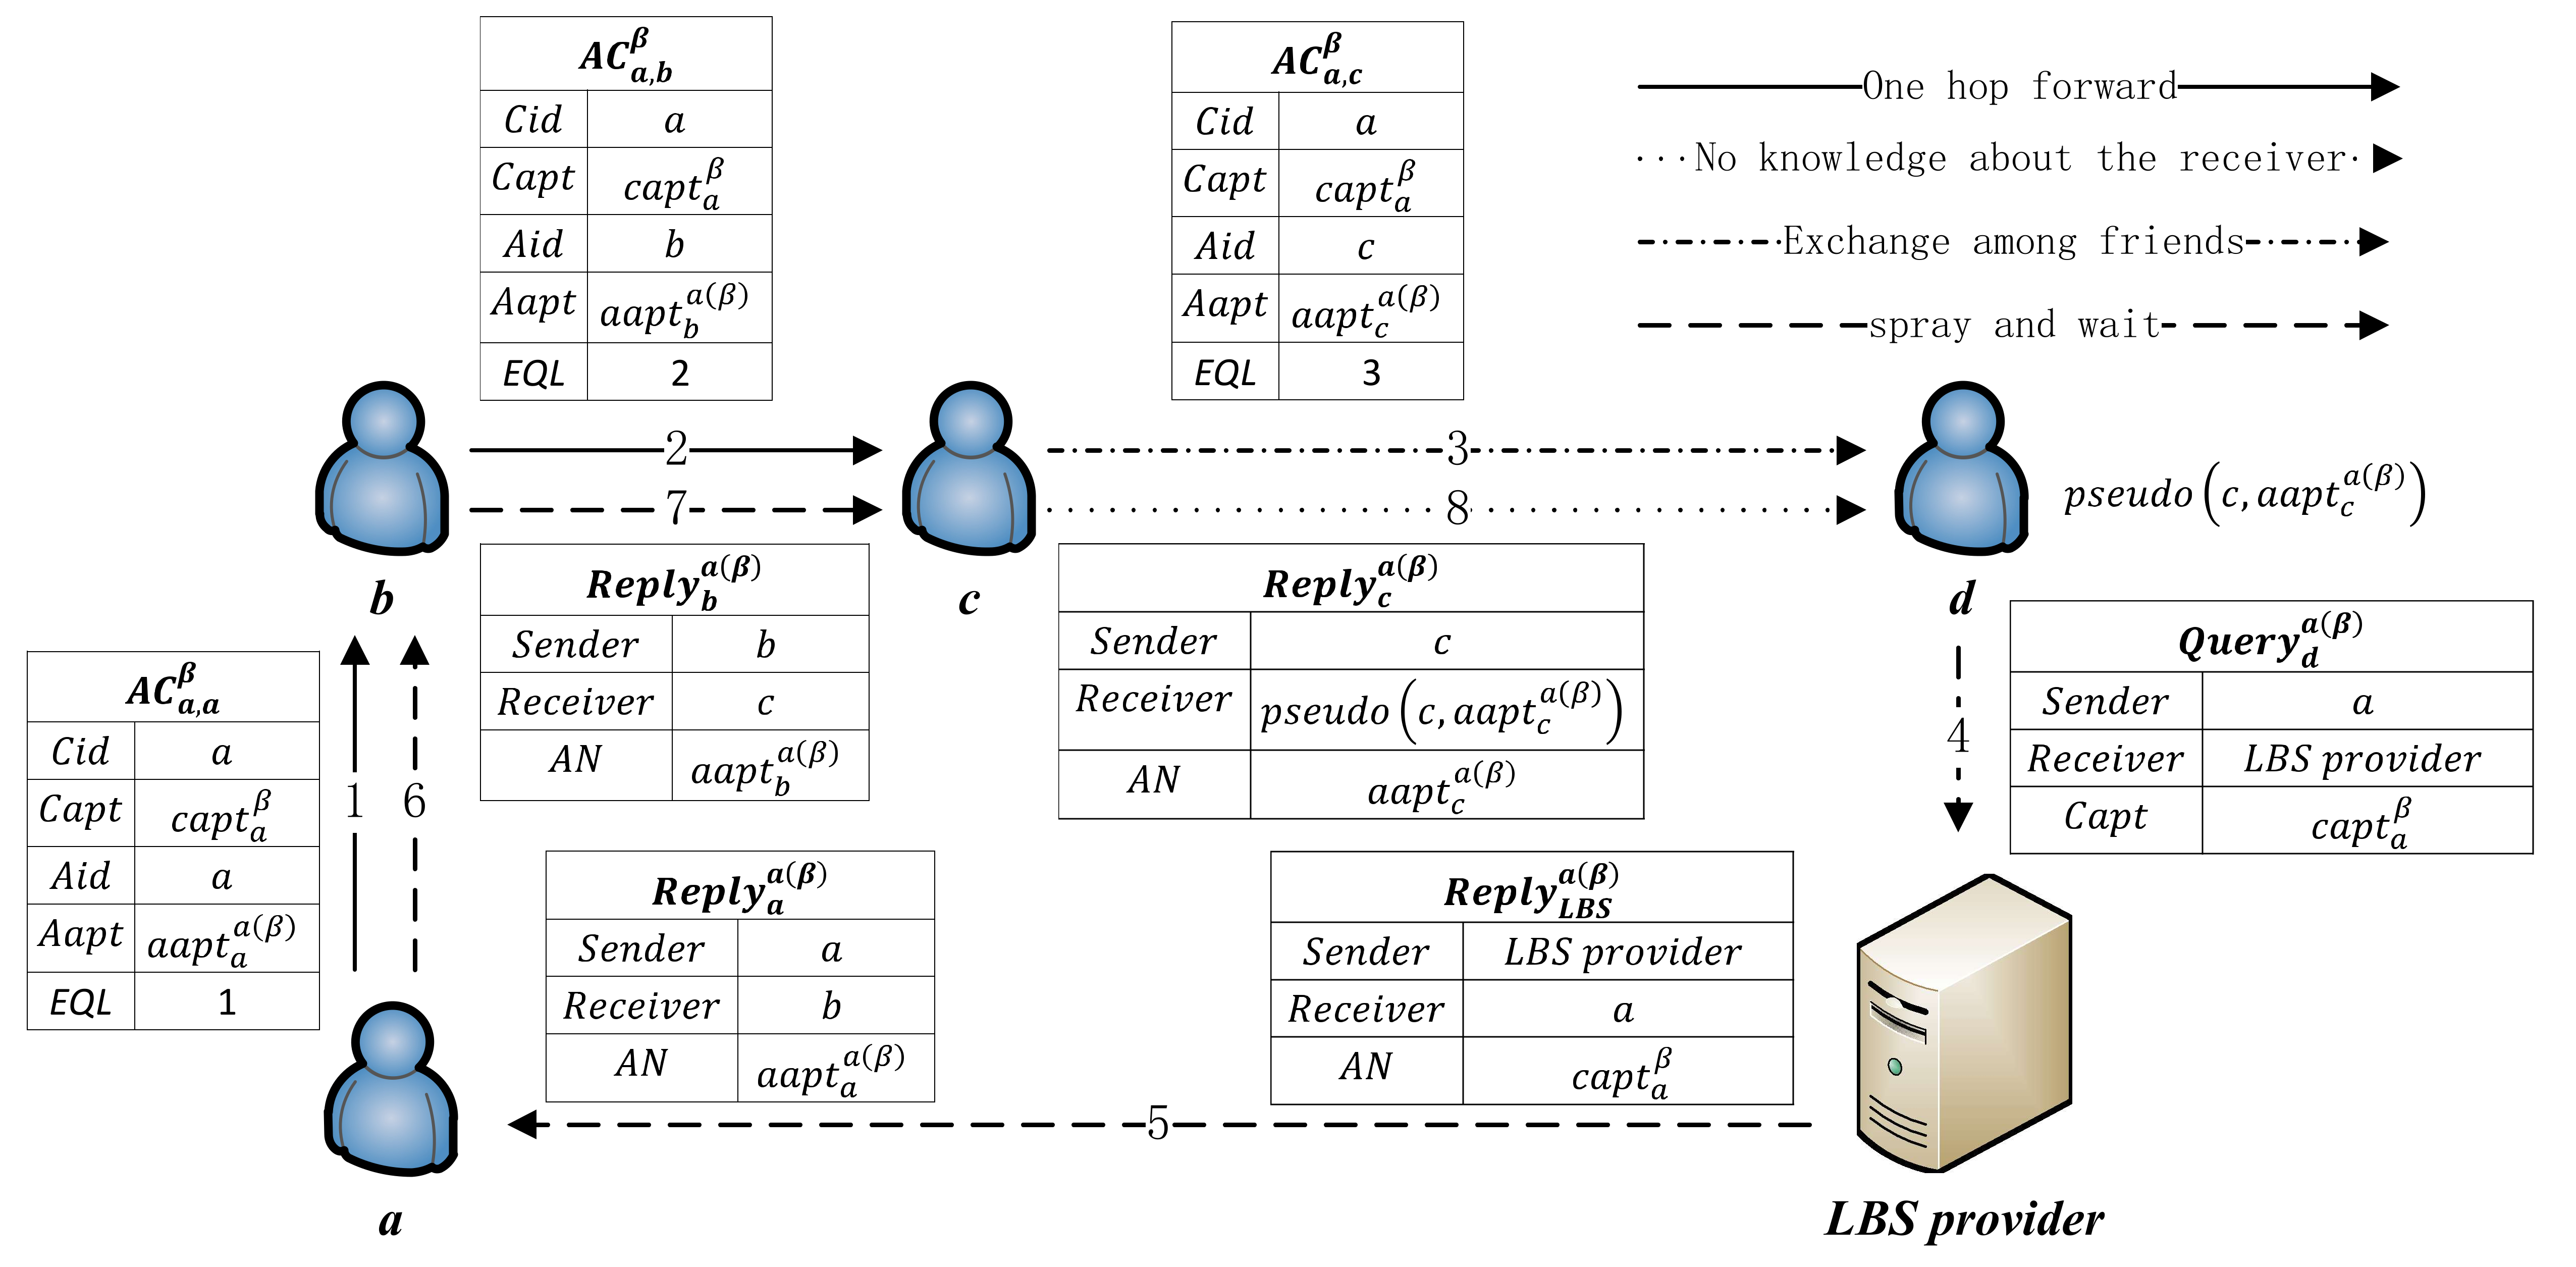
\includegraphics[width=6.0in]{figures/IEEEExampleofACPMessageExchange.png}
  \caption{Example of ACP Message Exchange} 
  \label{fig:EoACPME} %% label for entire figure 
\end{figure*}


Figure \ref{fig:EoACPME} is an example of the execution of the ACP protocol. Explanations of the symbols in the figure are shown in Table \ref{table:ACPSymbols}. These symbols and the figure are used throughout the paper to help us describe the protocol. For simplicity, we will omit some superscripts and subscripts from these symbols in the following sections when there is no ambiguity. The whole process can be considered as the following parts: 1) exchanging cards among all users who are called agents (i.e., 1 and 2), 2) exchanging cards among friends (i.e., 3), 3) sending query using information of appointment cards (i.e., 4), 4) forwarding the reply among agents (i.e., 5, 6 and 7), and 5) relaying to the original requester (i.e., 8). 


\begin{table} [hbtp]
\caption{ACP Symbols}
\label{table:ACPSymbols}
\centering
\tabulinesep=0.5mm
\begin{tabu} to 80mm{|X[1,c]|X[4,l]|} \hline 
%\begin{tabular}{|c|l|} \hline 
Parameter & Meanings \\ \hline 
${U}_{\varepsilon}$ & A user whose identity is $\varepsilon$. \\ \hline 
${AC}_{\alpha}^{\beta}$ & The $\beta^{th}$ appointment card generated by a user $\alpha$. \\ \hline 
${AC}_{{\alpha},{\gamma}}^{\beta}$ & ${AC}_{\alpha}^{\beta}$ is being forwarded by an agent $\gamma$. \\ \hline 
${Query}_{\delta}^{{\alpha}\left({\beta}\right)}$ & A query whose original requester is $\delta$ and using ${AC}_{\alpha}^{\beta}$ \\ \hline 
${{Reply}}^{{\alpha}\left({\beta}\right)}$ & The reply of a query which uses ${AC}_{\alpha}^{\beta}$. \\ \hline 
${{Reply}}_{\gamma}^{{\alpha}\left({\beta}\right)}$ & ${Reply}^{\alpha\left(\beta\right)}$ is being forwarded by an agent $\gamma$. \\ \hline 
${{Agt}}_{i}^{{\alpha}\left({\beta}\right)}$ & The $i^{th}$ ($i\geq1$) agent of ${AC}_{\alpha}^{\beta}$. \\ \hline 
${{capt}}_{\alpha}^{\beta}$ & The parameter $Capt$ in ${AC}_\alpha^\beta$. see Table \ref{table:AptCard} \\ \hline 
${{aapt}}_{\gamma}^{{\alpha}\left({\beta}\right)}$ & The parameter $Aapt$ in ${AC}_{\alpha}^{\beta}$, which is given by an agent $\gamma$. see Table \ref{table:AptCard} \\ \hline 
$AN$ & Both the $Capt$ and the $Aapt$ in an AC are called the Appointment Number. \\ \hline 
${NR}_{\varepsilon}$ & The number of \textit{ready}-ACs carried by ${U}_{\varepsilon}$ \\ \hline 
\end{tabu}
%\end{tabular}
\end{table}

\subsection{ Appointment Card}

To protect the original requester's location privacy, the original requester use others' identity (${Agt}_1$) to send queries to the LBSP instead of its own identity, so that the LBSP can reply to the original requester through ${Agt}_1$. Appointment cards make it possible for the agents to forward the reply to the original requester one by one. In other words, the appointment card indicates a path through which the original requestor can get its reply. 

In Figure \ref{fig:EoACPME}, the users \textit{a}, \textit{b} and \textit{c} are the agents of the appointment card ${AC}^{\beta }_a$ (i.e., ${Agt}^{a\left(\beta \right)}_1$, ${Agt}^{a\left(\beta \right)}_2$and ${Agt}^{a\left(\beta \right)}_3$). These agents are strangers, so the attackers can hardly infer $c$ from the identity of $a$. At the same time, $c$ is in the original requester $d$'s social tie (i.e.,$\ c$ is $d$'s friend or his friends' friend, so on), and he is the only one who knows how to reach $d$. Therefore, it is hard for attackers to infer the identity of $d$ from the identity of $a$. The appointment card is called a \textit{ready appointment card} (\textit{ready}-AC) after it leaves the last agent (i.e., the user $c$), or it is called the \textit{distributing appointment card} (simply \textit{distributing}-AC). It is obvious that \textit{distributing}-ACs are transmitted among agents who can be strangers, while a user can only get \textit{ready}-ACs from  one of his friends.

To make users carry a similar number of \textit{ready}-ACs, \textit{ready}-ACs are also exchanged between friends, so that a user can get \textit{ready}-ACs from his friends who have more \textit{ready}-ACs than him. As a result, the last agent is not sure whether the user who gets the \textit{ready}-AC from him is the original requester. We introduce a pseudonym mechanism, which enables the last agent to forward the reply to an unknown original requester. 

All users in the network are responsible for generating their respective ACs, and they are called the creators of their own ACs. The creator records his own identity ($Cid$) and a unique number ($Capt$) on his AC. When users exchange ACs, they modify $Aid$ (the agent ID) and ${Aapt}$ (the agent's appointment number) in the AC to enable the next agent to identify who is the predecessor. Entries of AC are shown in Table \ref{table:AptCard}.


\begin{table} [hbtp]
\caption{Appointment Card}
\label{table:AptCard}
\centering
\tabulinesep=0.5mm
\begin{tabu} to 80 mm {|X[1,c]|X[4,l]|} \hline 
%\begin{tabular}{|c|l|} \hline 
Parameter & Meanings \\ \hline 
$Cid$ & The identity of the creator who generates the AC.  \\ \hline 
$Capt$ & A unique number that distinguishes an AC from other ones generated by the same creator.   \\ \hline 
$Aid$ & The identity of an agent who gives the AC to the recent holder. (The previous hop of the AC)  \\ \hline 
$Aapt$ &  A unique number that distinguishes an AC from other ones transmitted by the same agent. \\ \hline 
$Timeout$ & The time when the AC expires.  \\ \hline 
\textit{EQ} & A queue (Exchange Queue) which records users who exchange the AC in order. Its length is \textit{EQL}.  \\ \hline 
\end{tabu}
%\end{tabular}
\end{table}


\subsection{ AC Life Cycle}

The life cycle of an AC starts when it is generated by its creator. The first $k$ (see Table \ref{table:ImptACSysParam}) agents add their identities into its Exchange Queue (\textit{EQ}) (see Table \ref{table:AptCard}) before exchanging it, which increases the length (\textit{EQL}) of the \textit{EQ}. When the AC's \textit{EQL} reaches $k$, it is eligible to be used in a query and is called a \textit{ready }AC. When an AC is used in a query, it is marked as an \textit{used} AC by the original requester who uses the AC. No matter what state (\textit{distributing}, \textit{ready} or \textit{used}) an AC is in, it can expire. An AC starts at the \textit{distributing} state. If the length of its \textit{EQ} reaches \textit{k}, it is switched to the \textit{ready} state. It can timeout in all states. When a user uses a \textit{ready} AC in a query, the AC is switched to the \textit{used} state. The user can also use the \textit{used} AC in other queries but he does not give the AC to anyone else. 

\subsection{ System Parameters}

All the system parameters are shown in Table \ref{table:ImptACSysParam}. 

\begin{table} [hbtp]
\caption{Important System Parameters}
\label{table:ImptACSysParam}
\centering
\tabulinesep=0.5mm
\begin{tabu} to 80 mm {|X[1,c]|X[4,l]|} \hline 
%\begin{tabular}{|c|l|} \hline 
Parameter & Meanings \\ \hline 
$k$ & The obfuscation distance \\ \hline 
$m$ & The friend obfuscation distance \\ \hline 
$GP$ & The generating period of appointment cards \\ \hline 
$Seg$ & The distributing segment \\ \hline 
$\tau$ & Avoiding time \\ \hline 
$AT$ & The timeout for appointment cards \\ \hline 
\end{tabu}
%\end{tabular}
\end{table}

\subsubsection{ Obfuscation Distance}

The obfuscation distance $k$ is the number of exchange before an AC is switched to the \textit{ready} state, and users who participate in the exchange are called agents, In other words, an AC must be exchanged $k$ times before it becomes a \textit{ready}-AC which can be used by a user in queries. Since the $k$ agents are strangers, the only relationship between two adjacent agents is that they encounter each other somewhere. The relationship between ${Agt}_1$ and ${Agt}_k$ becomes weaker when we increase $k$. In other words, attackers can hardly infer the identity of ${Agt}_k$ when they only knows the identity of ${Agt}_1$, and their difficulty increases with the increase of parameter $k$. As a result, it is hard for attackers to infer the original requester, even though ${Agt}_k$ is in the social tie of the original requester. Since the reply message must go through a series of agents, a long obfuscation distance also lengthens the path of the reply message. Therefore, a large $k$ makes the original requester safer, while making it harder and longer for the reply to be delivered.

\subsubsection{ Friends Obfuscation Distance}

Since ${Agt}_{k-1}$ is a stranger for ${Agt}_k$, it is possible that ${Agt}_{k-1}$ is exactly the attacker. We assume that the attacker knows that ${Agt}_k$ is in the social tie of the original requester. The attacker can assume that ${Agt}_k$ is a close friend of the original requester, so the identity of ${Agt}_k$ gives the attacker a good tip to infer the original requester. A solution to prevent the agent ${Agt}_{k-1}$ from learning the original requester easily is that the last $m$ ($1\leq m\leq k$) agents are friends, as shown in Figure \ref{fig:FriObfuscationDistance}. Here, $m$ is called \textit{friends obfuscation distance}, and the last $m$ agents are trusted agents.

\begin{figure} [hbtp]
  \centering 
  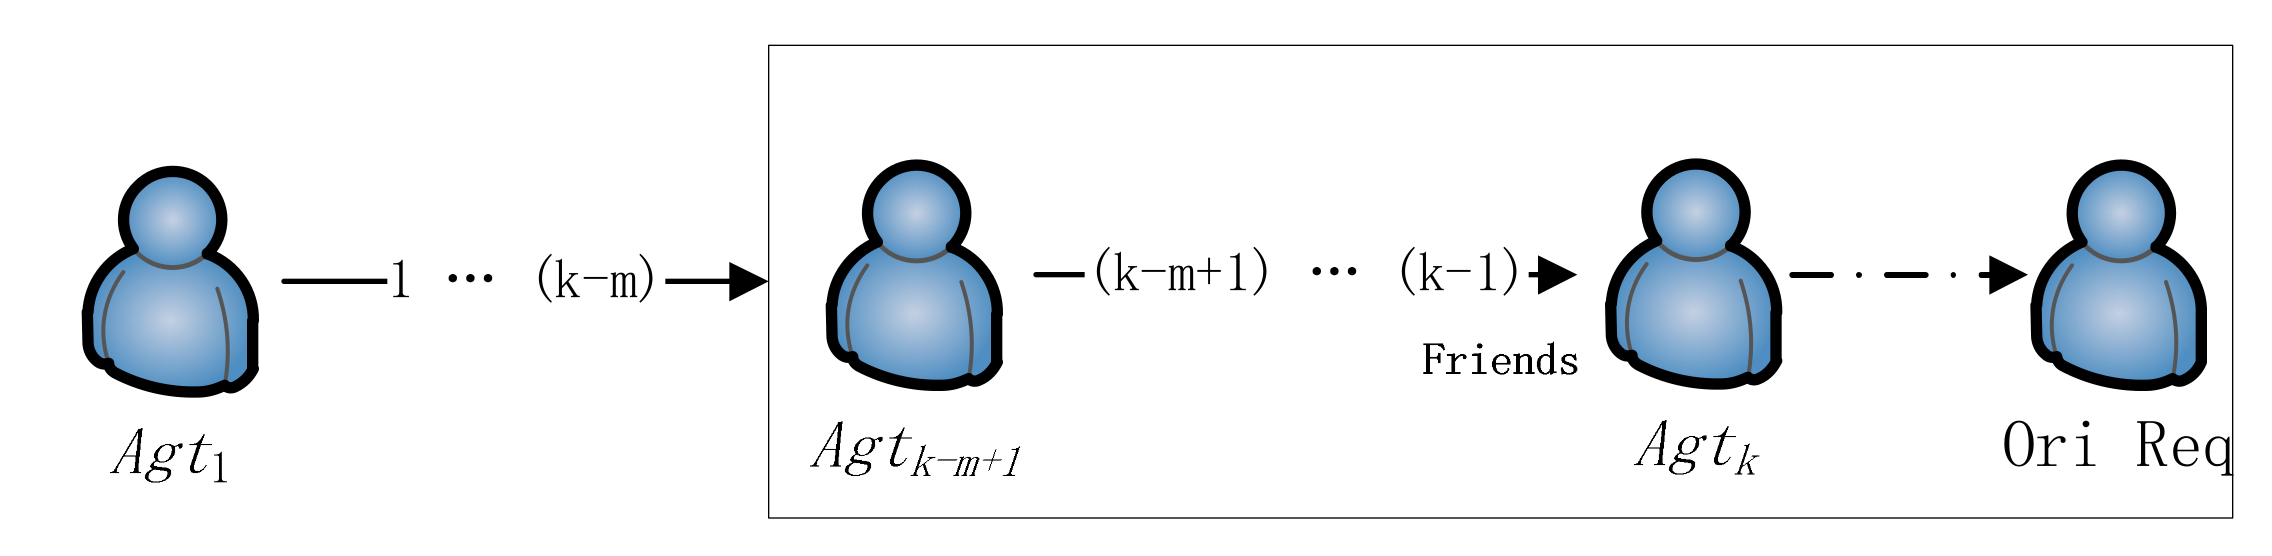
\includegraphics[width=3.5in]{figures/ACPFriObfDis.png}
  \caption{Friends-Obfuscation Distance} 
  \label{fig:FriObfuscationDistance} %% label for entire figure 
\end{figure}

However, friends encounter each other rarely, so having a large \textit{m} increases the difficulty of distributing ACs. In this paper, we assign $m$ to 1.

\subsubsection{ Generating Period}

Since ACs could expire, users must generate new ACs continuously. We use $GP$ to denote the speed of generating new ACs per user, that is, each user generates a new AC every $GP$ seconds.

\subsubsection{ Distributing Segment} \label{subsubsecDisSeg}

It is the stochastic serials of AC agents that increases the difficulty for attackers to infer the identity of the original requester. However, it is possible that many ACs are transmitted by the same serial of agents. We use the system parameter distributing segment, $Seg$, to avoid giving all \textit{distributing}-ACs to the same user. Each user maintains $Seg$ number of \textit{Distributing AC List}s (\textit{DL}s). It puts received \textit{distributing}-ACs in one of those \textit{DL}s randomly. If ${Agt}_i$ exchanges ACs with another user, ${Agt}_i$ selects one of his \textit{DL}s, and only ACs in that \textit{DL} will be exchanged with that user.

\subsubsection{ Avoiding Time} \label{subsubsecAvdTime}

Duplicated agents makes the obfuscation path of an AC less complicated. We use a parameter \textit{avoiding time,} $\tau$, to optimize the agent selection strategy. If a user gets an \textit{distributing}-AC at time $t_i$, he cannot get that \textit{distributing}-AC again before $t_i+\tau $.

\subsubsection{ AC Timeout}

Let $AT$ denote the timeout of ACs. An AC expires $AT$ seconds after it is generated. When an AC expires, all agents delete the AC information from their memory.

\subsection{ Protocol Details}


\subsubsection{ Generating Appointment Cards}

Maintaining a certain number of ACs in the network is a prerequisite for users for sending queries. Considering that ACs can expire, users must generate ACs continuously. The user who generates an AC is called the creator of the AC, at the same time, he is also the first agent of the AC. In our protocol, each user generates a new AC every $GP$ second. Since an AC has an $AT$-seconds timeout, there are $\delta =\frac{AT}{GP}$ appointment cards held by each user in the network. In other words, each user maintains about $\delta$ ACs which is generated by himself. Since users create ACs continuously, ACs have various timeouts so that it is likely for a user to pick an AC which does not expire in a long time (at least longer than his queries and replies).


\subsubsection{ Exchange Distributing Appointment Cards}\label{subsec_ExchangeDisAptCrd}

Users exchange their \textit{distributing}-ACs as frequently as possible, so that a \textit{distributing}-AC can be switched to a \textit{ready} one quickly. Still, there are some other conditions which should be satisfied when exchanging a \textit{distributing}-AC. Users should avoid giving all their \textit{ready}-ACs to a single user, which leads to identical serials of AC agents. As shown in subsection \ref{subsubsecDisSeg}, we use $Seg$ and \textit{DL}s to separate \textit{distributing}-ACs. We also need to prevent ACs from having duplicated agents using $\tau$ which is described in subsection \ref{subsubsecAvdTime}.

Let us take a pair of users Alice and Bob as an example. If Alice encounters another user Bob, Bob tells Alice whether he trusts her (Bob view her as a friend). Alice picks one of her \textit{distributing}-AC lists (e.g., \textit{DL}1). Alice traverses all ACs in \textit{DL}1 and \textit{distributing}-ACs which satisfy the following two conditions before exchanging them with Bob.

\begin{enumerate}
\item  If the length of the AC's \textit{EQ} (i.e., \textit{EQL}) is not shorter than $k-m$, then Alice must be a friend of Bob.

\item  Bob was not carrying the AC in the recent $\tau $ time interval.
\end{enumerate}

When Alice sends a \textit{distributing}-AC to Bob, she adds her identity and the current time to the AC's \textit{EQ}. Besides, Alice must modify the AC's $Aid\mathrm{\ }$to her own identity and its $Aapt$ to a new one. She also records the information in Table \ref{table:RelayTableEntries} as \textit{relay-table} in her memory. We should notice that the first agent (i.e., the creator) does not have a ${Aapt}_{old}$, because he is precisely the one who has generated the AC, in which case the ${Aapt}_{old}$ indicates his own identity. When Bob gets those ACs, he puts each one of the received \textit{distributing}-ACs to his \textit{DL}s respectively and randomly. If an AC whose \textit{EQL} is already equal to $k$, the AC must be switched to a \textit{ready} one when Bob gets it. Bob puts \textit{ready}-ACs on his \textit{ready}-AC list instead of \textit{distributing}-AC lists.

\begin{table} [hbtp]
\caption{Relay Table Entries}
\label{table:RelayTableEntries}
\centering
\tabulinesep=0.5mm
\begin{tabu} to 80 mm {|X[1,c]|X[4,l]|} \hline 
%\begin{tabular}{|c|l|} \hline 
Parameter & Meanings \\ \hline 
${Aapt}_{old}$ & The $Aapt$ generated by the previous agent \\ \hline 
${Aid}_{old}$ & The identity of the previous agent \\ \hline 
${Aapt}_{new}$ & The new $Aapt$ (generated by himself) \\ \hline 
${ID}_{nxt}$ & The identity of the next agent \\ \hline 
\textit{EQL} & The length of the AC's \textit{EQ} (should larger than 0) \\ \hline 
$AT$ & The time when the AC timeout. \\ \hline 
\end{tabu}
%\end{tabular}
\end{table}

\subsubsection{ Exchange Ready Appointment Cards}

Users ask for \textit{ready}-ACs only from their friends, which prevent strangers from learning the information of the users who are holding the \textit{ready}-ACs. The strategy of exchanging \textit{ready}-ACs should also meet some fairness criteria. That is, the number of each user's \textit{ready}-ACs should be more or less equal. 

Let us consider two friends Alice and Bob as an example. When Bob encounters Alice, Bob tells Alice the number of his \textit{ready}-ACs (${NR}_{Bob}$) and whether he wants Alice's \textit{ready}-ACs (if he trusts Alice). If Alice learns that Bob needs her \textit{ready}-ACs, she compares the number of her \textit{ready}-ACs (${NR}_{Alice}$) and ${NR}_{Bob}$. If ${NR}_{Bob}\ge {NR}_{Alice}$, Alice gives no \textit{ready}-AC to Bob; otherwise, she gives $\frac{{NR}_{Alice}-{NR}_{Bob}}{2}$ to Bob.

The process of exchanging \textit{ready}-ACs is much more straightforward than that for \textit{distributing}-ACs. Users do not modify any information in the \textit{ready}-ACs including $Aapt$ and $Aid$ so that the parameters of \textit{ready}-ACs always stay the same.

The algorithm of exchanging ACs when a user $U_i$ encounters another user $U_j$ is shown in Algorithm \ref{AlgExchACs}. The two users tell the other whether they are friends at the very beginning of their encounter. After they both know their relationship, they start to exchange their \textit{distributing}-ACs. When they both finish receiving the \textit{distributing}-ACs from the other, they continue to exchange their \textit{ready}-ACs at the same time. The process ends when they finish exchanging their \textit{ready}-ACs (or they do not need to exchange \textit{ready}-ACs).

\begin{algorithm} [hbtp]
\caption{Algorithm for exchanging ACs}\label{AlgExchACs}
\begin{algorithmic}[1]
\Procedure {Encounter} {$U_j$}
\If {$U_i$ trusts $U_j$}
	\State $U_i$ tells $U_j$ that $U_j$ is viewed as a friend.
\Else
	\State $U_i$ tells $U_j$ that $U_j$ is not viewed as a friend.
\EndIf
\State Wait for $U_j$ to tell $U_i$ whether $U_i$ is viewed as a friend.
\State $U_i$ chooses a distributing list (${DL}_{\omega}$) randomly.
\For {each ${AC}_u$ in ${DL}_{\omega}$}
	\If {$U_j$ was carrying ${AC}_u$ in the recent $\tau$ time}
		\State ${AC}_u$ cannot be sent to $U_j$
		\State continue (Try the next one.)
	\EndIf
	\If {the \textit{EQL} of ${AC}_u$ $\geq$ $k-m$}
		\If {$U_i$ is not trusted by $U_j$}
			\State ${AC}_u$ cannot be sent to $U_j$
			\State continue (Try the next one.)
		\EndIf
	\EndIf
	\State Send ${AC}_u$ to $U_j$
\EndFor
\State Tell $U_j$ that all \textit{distributing}-ACs are sent.
\State Receive all \textit{distributing}-ACs from $U_j$
\If {$U_i$ trusts $U_j$}
	\State $U_i$ tells $U_j$ ${NR}_i$.
\EndIf
\If {$U_i$ is trusted by $U_j$}
	\State Wait for $U_j$ to tell $U_i$ ${NR}_j$.
	\If {${NR}_j\geq{NR}_i$}
		\State send no \textit{ready}-AC to $U_j$
	\Else
		\State send $\frac{{NR}_i-{NR}_j}{2}$ number of \textit{ready}-ACs to $U_j$
	\EndIf
	\State Tell $U_j$ all \textit{ready}-ACs are sent.
\EndIf
\If {$U_i$ trusts $U_j$}
	\State Wait for \textit{ready}-ACs from $U_j$.
\EndIf 
\EndProcedure

\end{algorithmic}
\end{algorithm}

\subsubsection{ Sending Queries}

An original requester must send his queries to the LBSP and be able to get the reply from the LBSP while avoiding the LBSP from learning the identity of him. In ACP, the original requester sends his query using $Agt_1$'s identity to the LBSP, and $Agt_1$ is responsible for forwarding the reply from LBSP to the original requester. Therefore, the original requester's query includes a sender identity ${Agt}_1$, which is equal to the $Cid$ in the AC. Since ${Agt}_1$ needs a ${Capt}$ to identify the AC used by the query (and the reply), the ${Capt}$ in the AC is also in the query. The network can deliver that query to the destination LBSP efficiently with any DTN protocols.

We use the example in Figure \ref{fig:EoACPME}. The original requester $U_d$ has an AC (i.e., ${AC}^{\beta }_{a,c}$) whose creator is $U_a$. When $U_d$ uses it to send his query ${Query}^{a\left(\beta\right)}_d$, the sender identity is $a$, and the $Capt$ of the query is the $Capt$ of ${AC}^{\beta }_{a,c}$ (i.e., $capt_a^\beta$). The AC is marked as used when the query is ready to be sent so that the AC cannot be exchanged to other users. The original requester also uses a pseudonym to receive the reply, which is described in subsection \ref{paraLastAgent}. The algorithm that a user $U_i$ sends a query is shown in Algorithm \ref{AlgSendACPQuery}.


\begin{algorithm} [hbtp]
\caption{Algorithm for Sending Queries}\label{AlgSendACPQuery}
\begin{algorithmic}[1]
\Procedure {SendQuery } {}
\State Choose an \textit{ready}-AC, say ${AC}_{\alpha,f}^{\beta}$.
\State Assign the sender identity of the query to $U_{\alpha}$
\State Assign the receiver identity to the LBS
\State Assign the $AN$ to the ${capt}_{\alpha}^{\beta}$
\State Get a pseudonym $pseudo\left(U_f,{aapt}_f^{\alpha \left(\beta \right)}\right)$
\State Use the pseudonym as $U_i$’s identity.
\State Send the query to the LBS.
\EndProcedure
\end{algorithmic}
\end{algorithm}

\subsubsection{ Sending Replies}


\paragraph{ The LBSP part}

When the LBSP received the query, it learns that the sender's identity is the first agent $U_a$ instead of the original requester $U_d$, which protects the location privacy of the original requester. The LBS provider reply to the sender $U_a$, when it receives ${Query}^{a\left(\beta\right)}_d$. The reply also includes the $Capt$ of the query (i.e., $capt_a^\beta$), which enables $U_a$ to identify the AC used in the query and the reply.

\paragraph{ The First Agent}

When the first agent (i.e., ${Agt}_1$) gets the reply from the LBSP, he learns the $AN$ in the reply. He searches his \textit{reply-table} to get the information of the AC used in the query and reply. If the AC does not expire, there must be a corresponding entry in his \textit{reply-table}. It should be an entry where the $Aid_{old}$ and ${Aapt}_{old}$ are equal to ${Agt}_1$'s identity and the $AN$ of the reply, respectively. As a result, ${Agt}_1$ learns the identity of the next agent (i.e., ${Agt}_2$) from the ${ID}_{nxt}$ of the entry, so ${Agt}_1$ forwards the reply to ${Agt}_2$. The $AN$ of the reply is replaced with the ${Aapt}_{new}$ in the entry by ${Agt}_1$, which enables ${Agt}_2$ to identify the AC in ${Agt}_2$'s \textit{reply-table}.

For the example in Figure \ref{fig:EoACPME}, the first agent is $U_a$. When he receives ${Reply}^{a\left(\beta\right)}_{LBS}$, he learns that it is a reply from the LBS and the $Capt$ of the AC is ${capt}^{\beta}_a$. He searches his \textit{reply-table} for an entry whose ${Aid}_{old}$ is equal to $a$ and ${Aapt}_{old}$ is equal to ${capt}^{\beta }_a$. The ${ID}_{nxt}$ in the entry is equal to $b$ so he modifies the receiver of the reply message to $U_b$. $U_a$ also modifies the $AN$ in the reply message to ${aapt}^{a\left(\beta\right)}_a$ which is exactly equal to the ${Aapt}_{new}$ in his \textit{reply-table} entry, which enables $U_b$ identifies the AC in his \textit{reply-table}. 

\paragraph{ Intermediate Agents}

The process of forwarding replies in the intermediate agents (the second to the ${\left(k-1\right)}^{th}$ one) is similar to that of the first agent. We take the second agent as an example. When the second agent receives the reply forwarded by the first one, he learns the sender's identity (i.e., the first agent) and the $AN$ from the reply. In his \textit{reply-table}, there must be an entry which is related to the AC which is used in the reply (query), because he gets the AC from the previous agent. More specifically, his \textit{reply-table} must include an entry whose ${Aid}_{old}$ is equal to the previous agent's identity and the ${Aapt}_{old}$ is the value of $AN$ in the gotten reply.

For the example in Figure \ref{fig:EoACPME}, the second agent is $U_b$. When he receives ${Reply}^{a\left(\beta\right)}_a$, he learns that it is $U_a$ who forwards the reply message ${Reply}^{a\left(\beta\right)}_a$ and the $Aapt$ of the AC is ${aapt}^{a\left(\beta\right)}_a$. He searches his \textit{reply-table} for an entry whose ${Aid}_{old}$ is equal to $a$ and ${Aapt}_{old}$ is equal to ${aapt}^{a\left(\beta\right)}_a$. Since the ${ID}_{nxt}$ in the entry is equal to $c$, he modifies the receiver of the reply message to $U_c$. $U_b$ also modifies the $AN$ in the reply message to ${aapt}^{a\left(\beta\right)}_b$ which enables $U_c$ identifies the AC in his \textit{reply-table}, because the ${Aapt}_{new}$ in the entry is equal to ${aapt}^{a\left(\beta\right)}_b$. 

For each agent ${Agt}_i$, where $2\le i\le k-1$, he searches his \textit{reply-table} for a correlative entry, when he receives a reply. The ${Aid}_{old}$ and ${Aapt}_{old}$ in the entry should be equal to the sender's identity and the $AN$ in the reply. The identity of the next agent ${Agt}_{i+1}$ is ${ID}_{nxt}$. ${Agt}_i$ also assign ${Aapt}_{new}$ to the $AN$ in the reply to help ${Agt}_{i+1}$ search ${Agt}_{i+1}$'s \textit{reply-table}.

\paragraph{ The Last Agent} \label{paraLastAgent}

The last agent also searches for a \textit{reply-table} entry based on the reply, while he cannot get the identity of the next agent.

The last agent uses the same way to look up an entry in his \textit{reply-table} as the previous agents. When he finds that the \textit{EQL} is equal to $k$, he notices that he is the last agent. Then he is responsible for forwarding the reply to the original requester instead of another agent. He uses his identity and ${Aapt}_{new}$ in his \textit{reply-table} entry to generates a pseudonym

\begin{equation} \label{GrindEQ__ACPPsd} 
{psd}_{{Agt}_k}^{a\left( \beta \right)}=pseudo\left({Agt}_k,{Aapt}_{new}\right)
\end{equation}

, where the function $pseudo\left(id,Aapt\right)$ is a public pseudonym generating function which everyone in the network knows, including the original requester.

When the original requester sends his query, he also gets the same pseudonym ${psd}_{{Agt}_k}^{a\left( \beta \right)}$ using the pseudonym generating function. Note that he can get parameters from the AC. ${Agt}_k$ and ${Aapt}_{new}$ are equal to the $Aid$ and $Aapt$ in the AC. He uses that pseudonym as his identity before he gets the reply.

For the example in Figure \ref{fig:EoACPME}, the last agent is $U_c$. When he receives ${Reply}^{a\left(\beta\right)}_b$, he learns that it is $U_b$ who forwards the reply message ${Reply}^{a\left(\beta\right)}_b$ and the $Aapt$ of the AC is ${aapt}^{a\left(\beta\right)}_b$. He searches his \textit{reply-table} for an entry whose ${Aid}_{old}$ is equal to $b$ and ${Aapt}_{old}$ is equal to ${aapt}^{a\left(\beta\right)}_b$. Since the \textit{EQL} in the entry is equal to 3 (i.e. $k$), he recognizes that he is the last agent. $U_c$ calculates the pseudonym ${psd}^{a\left(\beta \right)}_c=pseudo\left(c,{aapt}^{a\left(\beta\right)}_c\right)$ then forward the reply to ${psd}^{a\left(\beta\right)}_c$. The original requester $d$ gets the identity $c$ and the ${aapt}^{a\left(\beta \right)}_c$ from the AC he uses, so that he uses the pseudonym ${psd}^{a\left(\beta \right)}_c$ as his identity. As a result, $U_d$ get the reply from $U_c$. The $AN$ of the reply is also assigned to ${aapt}^{a\left(\beta\right)}_c$ to avoid identical pseudonyms.

The algorithm of forwarding replies when an agent $U_i$ gets a reply message from $U_{prev}$ is shown in Algorithm \ref{AlgACPForwardReply}. $U_i$ learns the $AN$ and the identity of the sender from the reply message ${Reply}_{U_{prev}}^{\alpha\left(\beta\right)}$. Based on this information, $U_i$ checks his \textit{reply-table} to find out where the reply should be forwarded to, which is ${ID}_{nxt}$. After $U_i$ updates the $AN$ of the reply message, he forwards the reply message to ${ID}_{nxt}$.

\begin{algorithm} [hbtp]
\caption{Algorithm For Forwarding Replies}\label{AlgACPForwardReply}
\begin{algorithmic}[1]
\Procedure {Received} {${Reply}_{U_{prev}}^{\alpha\left(\beta\right)}$}
\State Get the $AN$ from ${Reply}_{U_{prev}}^{\alpha\left(\beta\right)}$
\If {$U_{prev}$ is the LBS}
	\State search $U_i$’s \textit{relay-table} to find an entry $E_i^{\alpha\left(\beta\right)}$
	\State whose ${Aapt}_{old}=AN$ and ${Aid}_{old}=U_i$
\Else
	\State search $U_i$’s \textit{relay-table} to find an entry $E_i^{\alpha\left(\beta\right)}$
	\State whose ${Aapt}_{old}=AN$ and ${Aid}_{old}=U_{prev}$	
\EndIf
\State Get the \textit{EQL}, ${Aapt}_{new}$ and ${ID}_{nxt}$ from $E_i^{\alpha\left(\beta\right)}$
\State Assign the $AN$ of ${Reply}_{U_{prev}}^{\alpha\left(\beta\right)}$ to ${Aapt}_{new}$.
\State Assign the sender identity to $U_i$.
\If {$EQL=k$}
	\State ${ID}_{nxt}\gets pseudo\left(U_i,{Aapt}_{new}\right)$
\EndIf
\State Forward the reply to ${ID}_{nxt}$
\EndProcedure

\end{algorithmic}
\end{algorithm}

\subsection{ Appointment Number}

The Appointment Number ($AN$) including $Capt$ and $Aapt$ is significant information in the AC. We explain the rules of generating them in detail and talk about the effect of ACs' timeout mechanism in this section.


\subsubsection{  Creator Appointment Number}

The Creator Appointment Number ($Capt$) is a number which is used to identify ACs generated by the same creator. In other words, if two ACs are generated by the same creator, and they do not expire, their $Capt$ must be different. Therefore, the first agent (i.e., the creator) cannot find two entries which have the same ${Aapt}_{old}$ in his \textit{reply-table}, if their ${Aid}_{old}$ are both his own identity.


\subsubsection{ Agent Appointment Number}

The Agent appointment number ($Aapt$) is a number used to identify appointment cards which have the same agent. Agents generate a new $Aapt$s for appointment cards before they exchange those cards to others. In other words, an agent gives any appointment card passing on by him a unique $Aapt$, which helps the next agent identify the appointment card in his \textit{reply-table}. Since the $Aapt$ is unique, an agent who is not the first one cannot find two entries which have the same pair of ${Aid}_{old}$ and ${Aapt}_{old}$, neither.

\section{ Experiment} \label{Experiment}

We used the map of Helsinki in our simulator to evaluate the performance of the proposed ACP. We also compare it to Binary Spray and Wait (BSW) protocol \cite{C19}, distributed social based location privacy protocol SLPD and our Multi-Hop Location-Privacy Protection (MHLPP) which is publishing. We simulated the continuous movement of users along streets on the map with one LBSP, fixed at a random location on the map.

For each user, we associate a random social value between 0 - 100\%, each corresponding to other users. Since each social value is assigned with equal probability, we can compute the expected number of friends of a user. If a user whose social value is larger than 85\% is called a friend and there are \textit{n} users in the network, there are $n\times \left(1-85\%\right)$ friends.

The Shortest Path Map-Based Movement (SPMBM) \cite{C22} is used in our experiment. For each experiment, we give the simulator a random seed so that it can generate a pseudo-random number based on the seed. Therefore, all the factors including users' speed and locations are the same if two experiments have the same random seed. All four protocols are tested using the same set of random seeds.

Before each experiment, the simulator runs for 800 seconds (simulator time). Then we pick 100 users out of 126 users randomly, and each of them sends a query to the LBSP. Tests last for about 20 minutes (simulator time). 


\subsubsection{  Average Query Success Ratio}

The query success ratio is the percentage of delivered queries among some attempts. Since users sending 100 queries in each experiment, if $s$ queries are delivered to the LBSP at time $t$, the query success ratio of time $t$ is $s\%$.

\begin{figure} [H]
  \centering 
  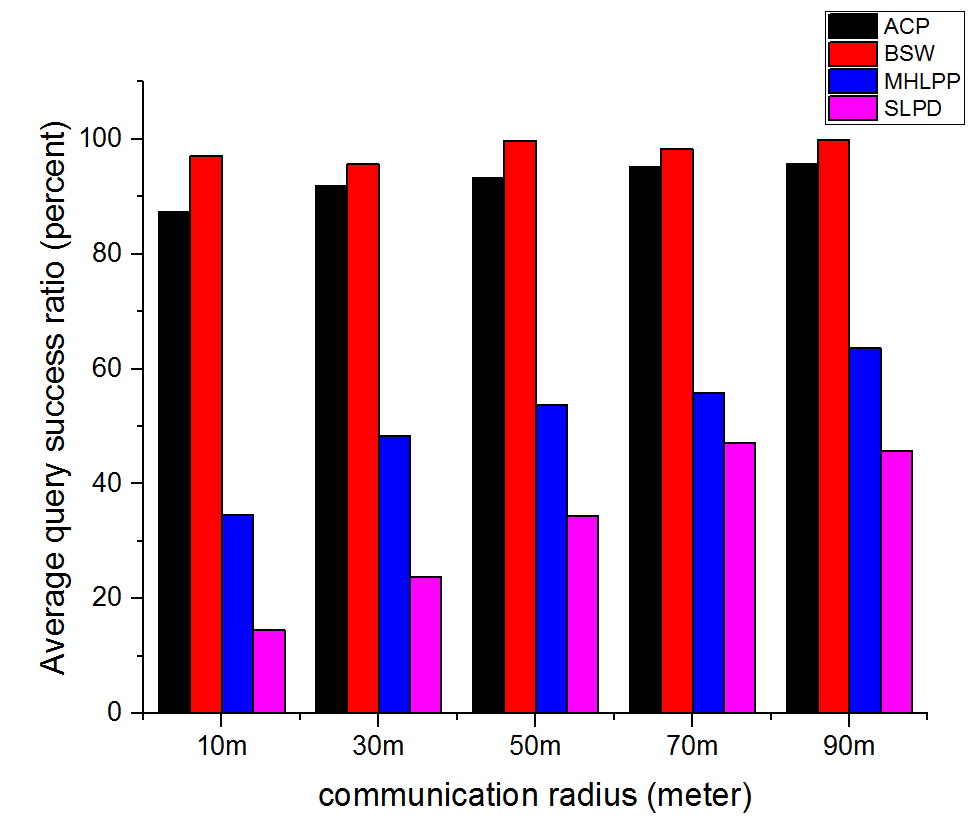
\includegraphics[width=2.6in]{figures/F414AverageQuerySuccessRatio10minutes.png}
  \caption{Average Query Success Ratio (10 minutes)} 
  \label{fig:AverageQuerySuccessRatio10} %% label for entire figure 
\end{figure}

As shown in Figure \ref{fig:AverageQuerySuccessRatio10}, we compare the average query success ratio of the four protocols with 5 kinds of communication radius (10, 30, 50, 70 and 90 meters). We observe that the ACP and the BSW get a high query success ratio, while the MHLPP and the SLPD are lower than the previous two protocols. The BSW is the highest one because it is a no-privacy protocol. The ACP is just a little lower than BSW, because the query delivery process of the ACP is almost the same as that of BSW. Since users of ACP must wait for available appointment cards, they cost more time to initial their queries. However, the ACP and the BSW are at the same level, comparing to the other two protocols. The MHLPP and the SLPD need to find friends to obfuscate their queries, which baffles their delivery process.


The experiment results when we test 20 minutes is shown in Figure \ref{fig:AverageQuerySuccessRatio20}. Comparing to the average query success ratio at 10 minutes, the MHLPP and the SLPD achieve much higher success ratio after 20 minutes than at 10 minutes. That is because it cost them so much time in their obfuscation phases when they need to find friends. In fact, some of the queries of the MHLPP and the SLPD still do not finish their obfuscation phase at 20 minutes.

\begin{figure} [H]
  \centering 
  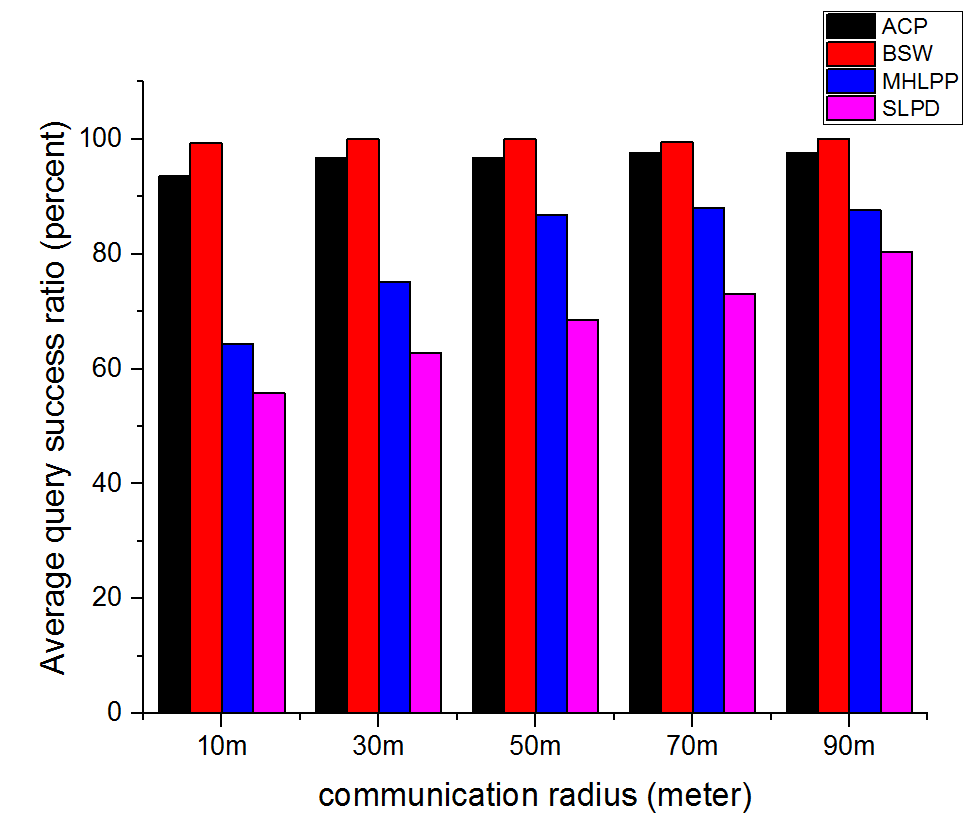
\includegraphics[width=2.6in]{figures/F415AverageQuerySuccessRatio20minutes.png}
  \caption{Average Query Success Ratio (20 minutes)} 
  \label{fig:AverageQuerySuccessRatio20} %% label for entire figure 
\end{figure}

The communication radius can influence the success ratio. In most of the cases, the success ratio rises when we increase the communication radius, and its influence is especially evident under 50 meters. A large communication radius makes it easy for users to encounter others, which is good for them to forward queries. However, a user who is so far away from the destination does not want the intermediates of his query encounters many users nearby. Because all users who carry copies of that query are near the sender instead of the destination, which decreases their query success ratio. Therefore, when the communication radius reaches 70 meters, the success ratios almost stay at the same level.

In Figure \ref{fig:F416AverageQuerySuccessRatioWith50MetersCommunicationRatio}, we observe that the ACP and the BSW have better convergence speed than the MHLPP and the SLPD. In other words, the former two protocols have a faster speed to approach the 100\% query success ratio than the latter two. At the very beginning, the ACP even has a little higher success ratio than the BSW. Because the ACP users need ready appointment card, and most of the users get their first ready appointment cards at places where there are many users. Therefore, users rarely generate query near the edges of the map at the beginning, which facilitates their queries delivery process. For example, if a user generates his query at the edge of the map, the copies of this query might be sent to users who are also at the edge, and it takes more time for them to deliver the query. If the user does not generate his query until he arrives a place nearer the center, the copies of this query will be carried by the users in the center with higher probability.

\begin{figure} [hbtp]
  \centering 
  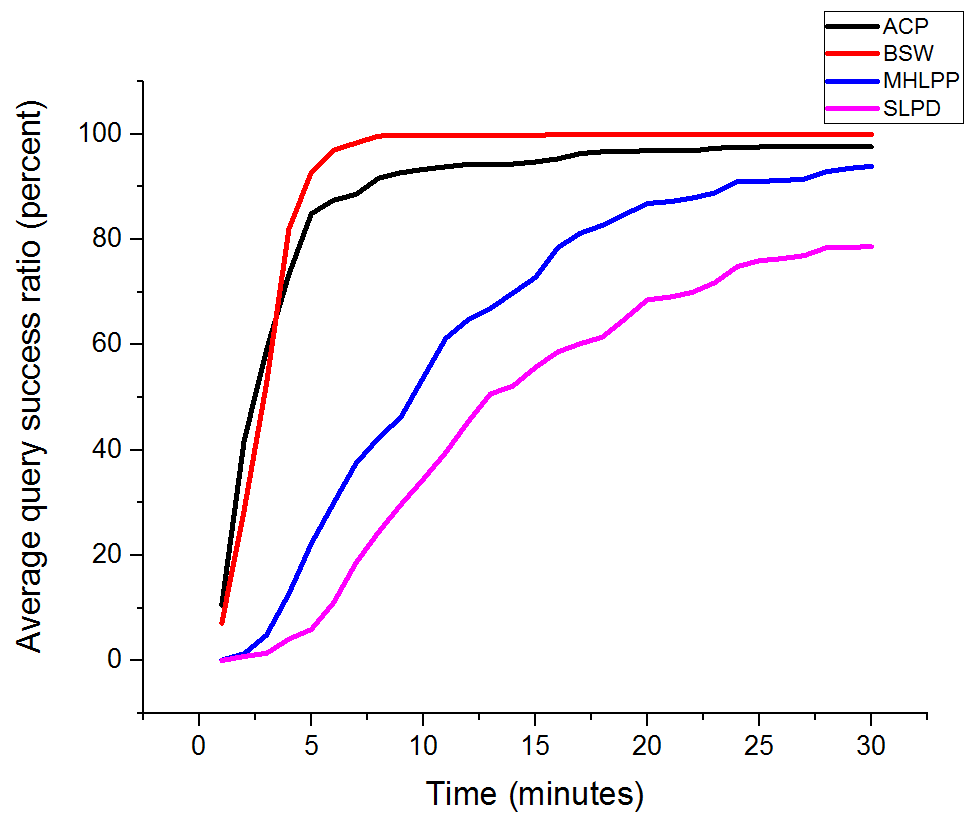
\includegraphics[width=2.6in]{figures/F416AverageQuerySuccessRatioWith50MetersCommunicationRatio.png}
  \caption{Average Query Success Ratio With 50-Meters Communication Ratio} 
  \label{fig:F416AverageQuerySuccessRatioWith50MetersCommunicationRatio} %% label for entire figure 
\end{figure}

\subsubsection{ Average Reply Success Ratio}

When the LBSP receives a query, it sends a reply to the requester. If the reply arrives the original requester before the test ends, we view it as a success; otherwise, the reply is failed. There are two reasons for the failure of replies: 1) the query is not delivered to the LBSP successfully; 2) the query costs too much time so that the reply has no time to be delivered; 3) The route of the reply is too long. Since there are 100 queries in each experiment, the number of replies should be equal to 100. 

In Figure \ref{fig:F417AverageReplySuccessRatioWith50MetersCommunicationRatio}, the BSW has a significant and reasonable higher success ratio than all other protocols, because it is a no-privacy protocol. The ACP is higher than the MHLPP and the SLPD, but its advantage is not as large as that in the query process. In fact, the reply process of the MHLPP and the SLPD are simpler than that of the ACP, but the ACP saves so much time in its query process that it earns a better reply success ratio than the other two.

\begin{figure} [hbtp]
  \centering 
  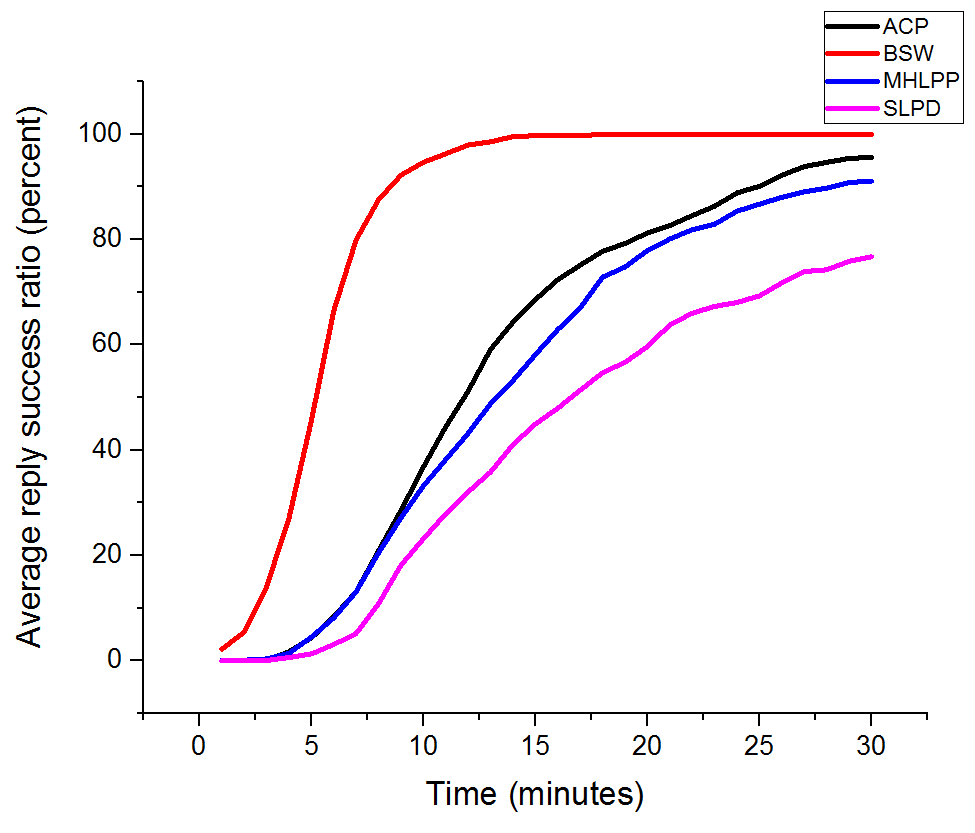
\includegraphics[width=2.6in]{figures/F417AverageReplySuccessRatioWith50MetersCommunicationRatio.png}
  \caption{Average Reply Success Ratio With 50-Meters Communication Ratio} 
  \label{fig:F417AverageReplySuccessRatioWith50MetersCommunicationRatio} %% label for entire figure 
\end{figure}

\subsubsection{ Total Number of Query Relays}

The query delivery processes of all the four protocols use the BSW protocol, and the BSW makes copies for queries and gives half of the copies to any users it encounters. That is a significant cost for the network, so we use the number of query relaying (QR) to evaluate that cost. The QR is initialized as zero at the beginning of the test. When a user relay a (or several) copies of a query, we increase QR by 1. For example, in the SLPD, there are two phases: the obfuscation phase and the free phase. In the obfuscation phase, a query is forwarded among one-hop friends for $k$ times. After that, it is forwarded by the BSW protocol. The BSW protocol makes $c$ copies of the query and gives half of the copies to any encountering users. Then QR should be about $k+c$. Since a user gives all its copies to the destination if he encounters the destination at once, the QR may be smaller. The smaller that number is, the smaller cost of the network is. Since there are 100 queries, we divide QR by 100 to get an average value. 

In Figure \ref{fig:F418AverageTotalNumberofForwardingQueriesAt20Minutes}, we compare QR with four protocols. We observe that all the four protocols are at a similar level, the BSW and the ACP is a little lower than the other two. For the ACP and the BSW, they deliver queries so fast that users who carry more than one copies give all their copies to the destination before they send these copies to different users separately. As a result, many copies have no chance to be forwarded, which decreases the cost. While the MHLPP and the SLPD have obfuscation phases, the queries start to be delivered freely (in a BSW way) at a random place where might be so far away from the destination, so that almost all copies can be forwarded respectively.

\begin{figure} [hbtp]
  \centering 
  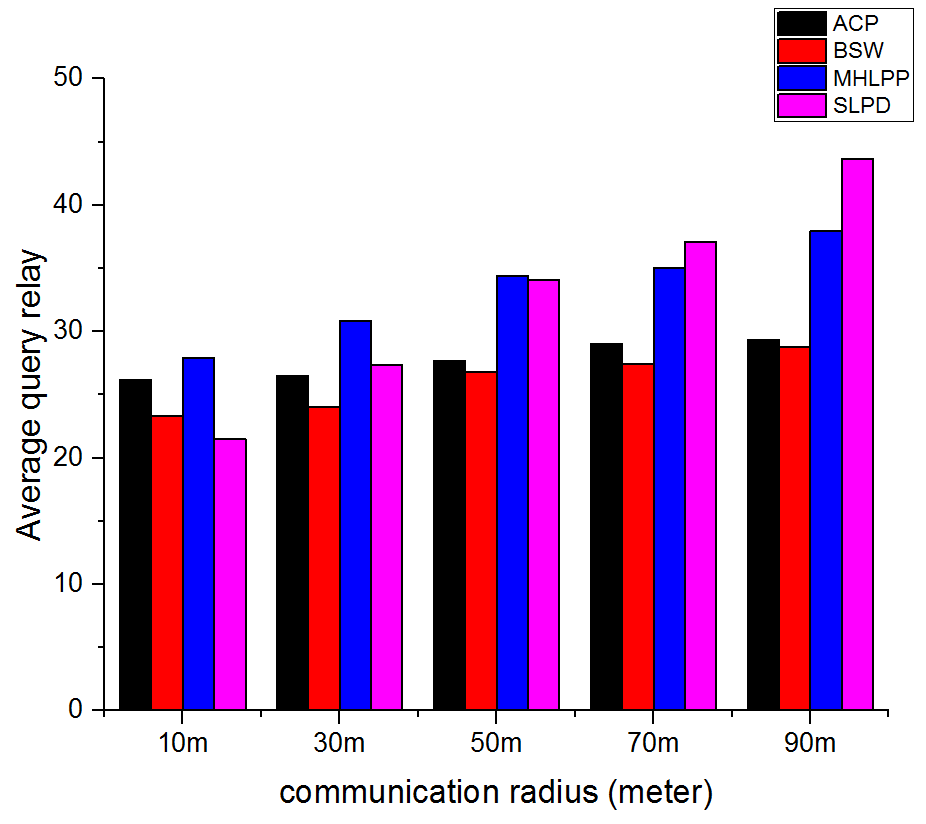
\includegraphics[width=2.6in]{figures/F418AverageTotalNumberofForwardingQueriesAt20Minutes.png}
  \caption{Average Total Number of Forwarding Queries At 20 Minutes} 
  \label{fig:F418AverageTotalNumberofForwardingQueriesAt20Minutes} %% label for entire figure 
\end{figure}

The communication radius affects the total number of the forwarding queries, especially for the MHLPP and the SLPD. Those two protocols can finish their obfuscation phase more quickly which a larger communication radius, so that more queries can be forwarded freely (in the BSW way), which makes their QR larger.

\subsubsection{ Memory Cost}

We count the number of queries carried by each user to evaluate the memory cost of the four protocols. Several copies of a query are counted for only once.

In the Figure \ref{fig:F419AverageQueryBufferNeededAt20Minutes}, we compare the number of queries per user with the four protocols at 20 minutes. We observe that the BSW is the highest in most of the cases and the ACP always stays at a similar level as the BSW. The data of other two protocols (the MHLPP and the SLPD) increase as the communication radius. The MHLPP even excesses the BSW when the communication radius is 90 meters. The reason is that quite a number of the BSW and the ACP users forward their copies to the destination so that there is no copy with them at 20 minutes, while the rest of them cannot forward their copies to the destination even given a large communication radius. At the same time, the number of the other two protocol's free phase queries is significantly influenced by the communication radius. The more queries are in the free phase; the more copies are in the network.

\begin{figure} [H]
  \centering 
  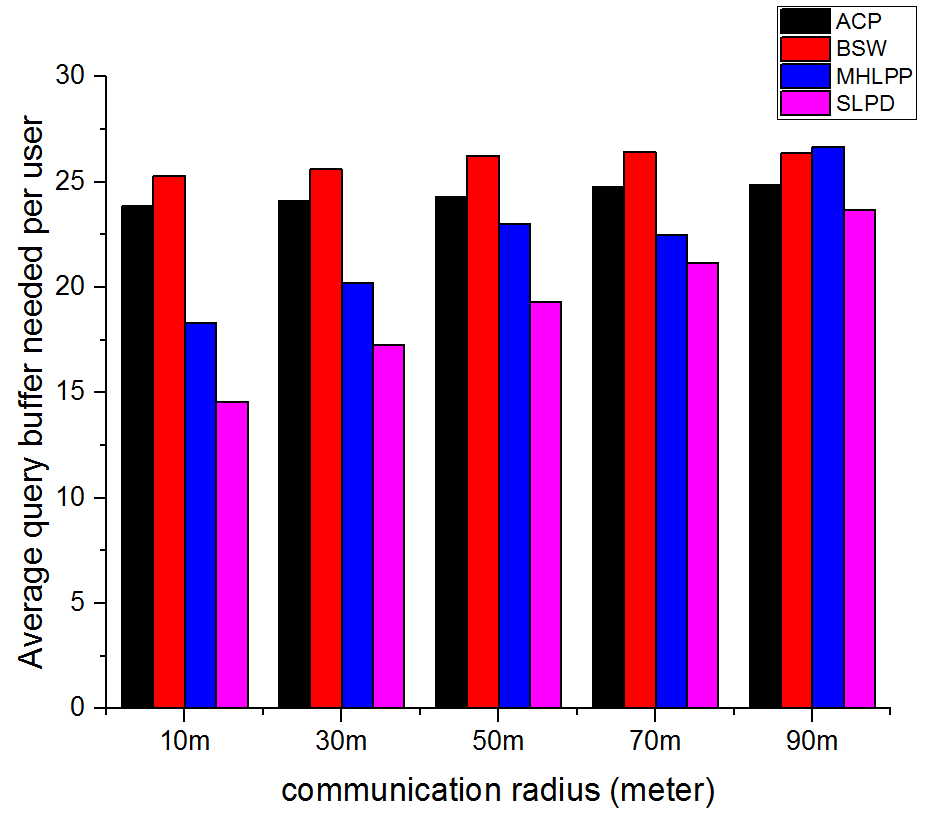
\includegraphics[width=2.6in]{figures/F419AverageQueryBufferNeededAt20Minutes.png}
  \caption{Average Query Buffer Needed At 20 Minutes} 
  \label{fig:F419AverageQueryBufferNeededAt20Minutes} %% label for entire figure 
\end{figure}

The Figure \ref{fig:F420AverageNumberofCarriedQueriesPerUser} shows the average number of queries which are carrying by users when the communication radius is 10, 50 and 90 meters. The curves of the ACP and the BSW rise sharply at the beginning and then become flat, while those of the MHLPP and the SLPD rise smoothly and continuously. 

\begin{figure} [H]
  \centering 
  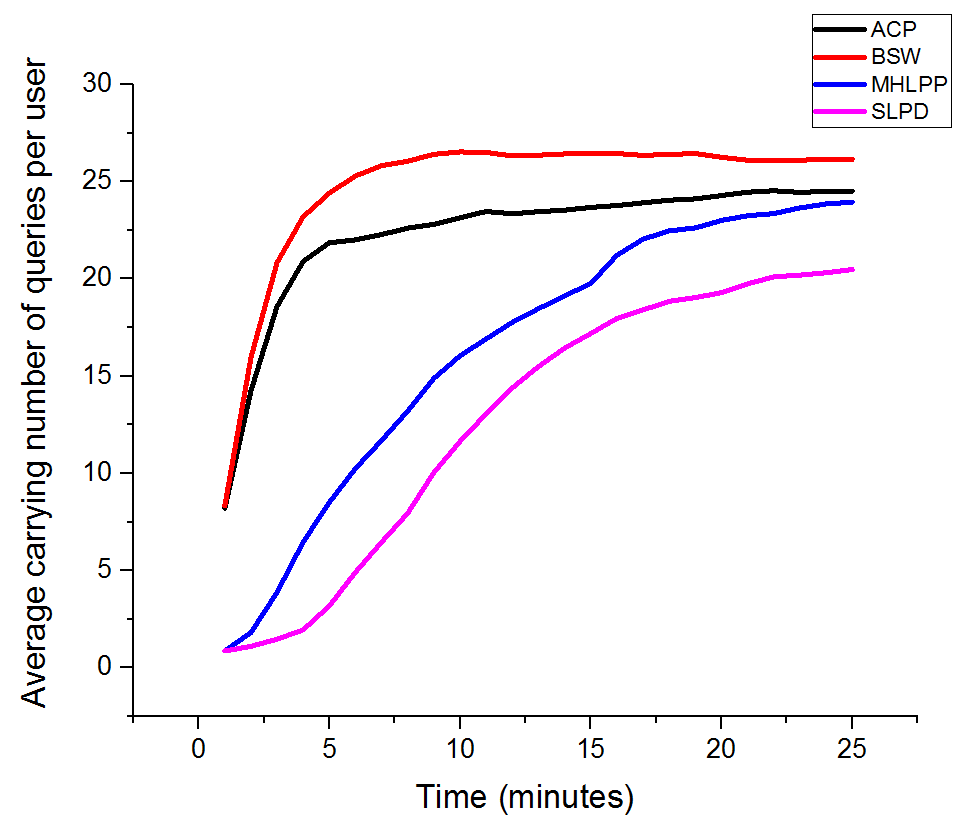
\includegraphics[width=2.6in]{figures/F420AverageNumberofCarriedQueriesPerUser50.png}
  \caption{Average Number of Carried Queries Per User (communication radius 50 meters)} 
  \label{fig:F420AverageNumberofCarriedQueriesPerUser} %% label for entire figure 
\end{figure}

\subsubsection{ Distributing Appointment Cards}

Exchanging appointment cards is a feature of the ACP, which imports burden into the network. We count the number of exchanging appointment cards per minute to evaluate the extra cost of the ACP.

In Figure \ref{fig:F422AverageNumberofExchangingACsPerMinute}, we count the total number of exchanging ACs in the whole network. For example, if a user Alice encounters another user Bob, the total of exchanging ACs processes increases by one when Alice exchanges any ACs to Bob. We count the number of those exchanging processes occur per minute. As shown in the figure, the exchanging processes do not occur frequently, but about 2 times per minutes. Since the size of an appointment card is small, it does not cost the network many resources.

\begin{figure} [hbtp]
  \centering 
  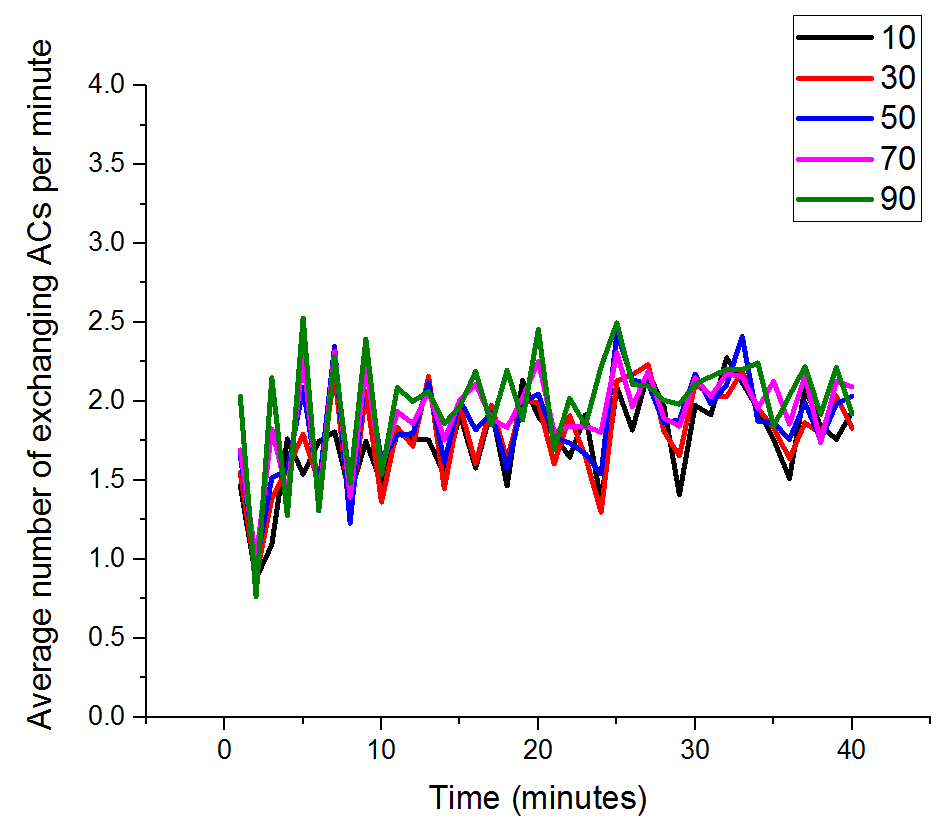
\includegraphics[width=2.6in]{figures/F422AverageNumberofExchangingACsPerMinute.png}
  \caption{Average Number of Exchanging ACs Per Minute} 
  \label{fig:F422AverageNumberofExchangingACsPerMinute} %% label for entire figure 
\end{figure}

\section*{Conclusion}

The location privacy-preserving protocol ACP uses social-relationship. It facilitates the obfuscation process by continuously exchanging appointment cards among users so that the original requester does not communicate with any of his friends when he sends a query. Simulation results show that it has a better performance with respect to the query-delivery success ratio and provides an acceptable obfuscation compared to its counterparts. Although ACP requires more time to forward the reply, the total time required for query delivery and reply delivery is still less than that for its counterparts SLPD and MHLPP. The major disadvantage is that the ACP must exchange ACs continuously, which can consume network resources. However, that cost is low if users do not send too many queries.

%\section*{References}

\begin{thebibliography}{00}

\bibitem{C1} K. Fall, ``A Delay-Tolerant Network Architecture for Challenged Internets,'' in Proceedings of the Conference on Applications, Technologies, Architectures, and Protocols for Computer Communications, pp. 27-34, 2003.
\bibitem{C2} J. Schiller, A. Voisard, ``Location-Based Services,'' Morgan Kaufmann, 2004.
\bibitem{C3} M. Gruteser, D. Grunwald, ``Anonymous Usage of Location-Based Services Through Spatial and Temporal Cloaking,'' in Proceedings of the 1st International Conference on Mobile Systems, Applications and Services, pp. 31-42, 2003
\bibitem{C4} S. Zakhary, M. Radenkovic, ``Utilizing social links for location privacy in opportunistic delay-tolerant networks,'' in Proceedings of International Conference on Communications (ICC), 2012.
\bibitem{C5} S. Zakhary, M. Radenkovic, A. Benslimane, ``The quest for location-privacy in opportunistic mobile social networks,'' in Proceedings of IWCMC, 2013.
\bibitem{C6} S. Zakhary, M. Radenkovic, A. Benslimane, ``Efficient Location Privacy-Aware Forwarding in Opportunistic Mobile Networks,''  IEEE Trans. on Vehicular Technology, Vol. 63, No. 2, pp. 893 – 906, 2014.
\bibitem{C7} E. Daly, M. Haahr, ``Social Network Analysis for Routing in Disconnected Delay-Tolerant MANETs,'' in Proceedings of the 8th ACM International Symposium on Mobile Ad Hoc Networking and Computing, 2007.
\bibitem{C8} M. Duckham, ``Moving forward: Location privacy and location awareness,'' in Proceedings of the 3rd ACM International Workshop on Security and Privacy in GIS and LBS, pp. 1-3, 2010.
\bibitem{C9} T. Hashem, L. Kulik, ``Safeguarding location privacy in wireless ad-hoc networks,'' in Proceedings of  UbiComp, pp. 372-390,  2007.
\bibitem{C10} L. Sweeney, ``k-Anonymity: A Model for Protecting Privacy,'' International Journal on Uncertainty,. Fuzziness and Knowledge-based Systems, Vol. 10, No. 5, pp. 557-570, 2002. 
\bibitem{C11} M. Mano, Y. Ishikawa, ``Anonymizing User Location and Profile Information for Privacy-aware Mobile Services,'' in Proceedings of the 2nd ACM SIGSPATIAL International Workshop on Location Based Social Networks, pp 68-75, 2010.
\bibitem{C12} T. Wang, L. Liu, ``Privacy-aware mobile services over road networks,'' in Proceedings of the VLDB Endowment, pp. 1042-1053, Vol. 2,  2009.
\bibitem{C13} R. Lu, X. Lin, X. Shen, ``SPRING: A Social-based Privacy-preserving Packet Forwarding Protocol for Vehicular Delay Tolerant Networks,'' in Proceedings of IEEE INFOCOM, 2010.
\bibitem{C14} J. Zhang, C. Chow, ``REAL: A Reciprocal Protocol for Location Privacy in Wireless Sensor Networks,'' IEEE Trans. on Dependable and Secure Computing, Vol. 12, No. 4, pp. 458 – 471, 2015.
\bibitem{C18} R. Xiang, J. Neville, M. Rogati, ``Modeling Relationship Strength in Online Social Networks,'' in Proceedings of the 19th International Conference on World Wide Web, pp 981-990, April 26 - 30, 2010.
\bibitem{C19} T. Spyropoulos, K. Psounis, C. S. Raghavendra, ``Spray and Wait: An Efficient Routing Scheme for Intermittently Connected Mobile Networks,'' in Proceedings of the ACM SIGCOMM Workshop on Delay-tolerant Networking, pp. 252-259, 2005.
\bibitem{C20} B. Ying, A. Nayak, ``Social Location Privacy Protection Method in Vehicular Social Networks,'' in Proceedings of 5th IEEE International Workshop on Smart Communication Protocols and Algorithms, May 21-25 2017.
\bibitem{C21} B. Ying, A. Nayak, ``Location Privacy-protection based on p-destination in mobile social networks: A game theory analysis,'' in Proceedings of IEEE International Conference on Dependable and Secure Computing, Aug. 7-10 2017.
\bibitem{C22} A. Keränen, J. Ott, and T. Kärkkäinen, ``The ONE simulator for DTN protocol evaluation,'' in Proc. of SIMUTools, 2009.
\bibitem{C23} J. Krumm, ``A survey of computational location privacy,'' Personal and Ubiquitous Computing, Volume 13, Issue 6, pp 391-399, 2009.
\bibitem{C24} A.K. Pietiläinen, ``Opportunistic Mobile Social Networks at Work''. Ph.D. Thesis, Université Pierre et Marie Curie, Paris, 2010.
\end{thebibliography}




\end{document}
